\documentclass[hidelinks,aspectratio=169]{beamer}
\usepackage[italian]{babel} 
\usepackage[utf8]{inputenc} 
\usepackage{fourier} 

%Slide colors
\usetheme{Madrid}
%\usecolortheme{beaver}

% Images
\usepackage{graphicx}
\usepackage{caption}
\usepackage{subcaption}
\usepackage{float}
\graphicspath{{Immagini}}

% Stop hyphenation
\usepackage[none]{hyphenat}

% Minipages in the same line
\usepackage{tabularx}

% Coloring links
\usepackage{xcolor}

% Enumerate abc
\usepackage{enumerate}

% Redefines caption setup in way to remove "Figure:"
\usepackage{caption}
\captionsetup[figure]{labelformat=empty}

% To set element positions
\usepackage{ragged2e}

% To insert the logo in the bottom right conrner
\usepackage{tikz}

% License
\usepackage[
type={CC},
modifier={by-nc-sa},
version={4.0},
]{doclicense}

%------------------- Commands zone --------------------

%Command to zoom in
\usepackage{mwe}
\makeatletter
\newsavebox\zb@x
\newcounter{z@@m}
\usepackage{calc}
\newdimen\B@r\newdimen\P@r
\newdimen\@zw\newdimen\@zh\newdimen\@zd

\newcommand{\zoombox}[2][0]{%
	\leavevmode%
	\sbox\zb@x{#2}%
	\setlength\B@r{1pt*\ratio{\wd\zb@x}{\ht\zb@x+\dp\zb@x}}%
	\setlength\P@r{1pt*\ratio{\paperwidth}{\paperheight}}%
	\ifdim\B@r>\P@r\relax%
	\setlength\@zw{\wd\zb@x}\setlength\@zh{\@zw*\ratio{\paperheight}{\paperwidth}}%
	\setlength\@zd{(\@zh-\ht\zb@x-\dp\zb@x)*\real{0.5}+\dp\zb@x}%
	\setlength\@zh{\@zh-\@zd}%
	\else%
	\setlength\@zh{\ht\zb@x+\dp\zb@x}%
	\setlength\@zw{\@zh*\ratio{\paperwidth}{\paperheight}}%
	\setlength\@zh{\ht\zb@x}\setlength\@zd{\dp\zb@x}%
	\fi%
	\makebox[0pt][l]{\makebox[\wd\zb@x][c]{\makebox[\@zw][l]{%
				\pdfdest name {zbfs\thez@@m} fitr
				width  \@zw\space
				height \@zh\space
				depth  \@zd\space
	}}}%
	\pdfdest name {zb\thez@@m} fitr
	width  \wd\zb@x\space
	height \ht\zb@x\space
	depth  \dp\zb@x\space
	\immediate\pdfannot 
	width  \wd\zb@x\space
	height \ht\zb@x\space
	depth  \dp\zb@x\space
	{%
		/Subtype/Link/H/N
		/Border [0 0 #1 [1 2]]
		/A <<
		/S/JavaScript
		/JS (
		if(typeof(zoomed)=='undefined'||!zoomed){
			var lastView=this.viewState;
			if(app.fs.isFullScreen) this.gotoNamedDest('zbfs\thez@@m');
			else this.gotoNamedDest('zb\thez@@m');
			zoomed=true;
		}else{
			this.viewState=lastView;
			zoomed=false;
		}
		)
		>>
	}%
	\usebox{\zb@x}%
	\stepcounter{z@@m}%
} 
\makeatother

%------------------- Header --------------------
\title[]{\textbf{Think in 3-D} \\ \vspace*{3mm} \small \textbf{Tecnologie 3-D per riparazioni e sostituzioni personalizzate di componentistica}}
\author[Think in 3-D]{}
\date{}
\logo{\includegraphics[scale=0.1]{logo_bianco.png}}

\begin{document}
	
	\begin{frame}[plain]
		\maketitle
		\vspace*{-20mm}
		\begin{center}
			\hspace*{3mm}
			\textbf{Presentazione del progetto per il Contamination Lab}
			
			\vspace*{5mm}
			%\newline 
			\begin{tabularx}{\linewidth}{XXX}
				{
				\hspace*{20mm}
				\zoombox{\includegraphics[scale=0.2]{logo_bianco.png}}
				}&{
				\hspace*{8mm}
				\zoombox{
\includegraphics[scale=0.2]{logo-uniurb-2016.jpg}}
				}&{
				\hspace*{10mm}
				\zoombox{
\includegraphics[scale=0.2]{Logo_contamination.png}}
				}
			\end{tabularx}
		
		\vspace{5mm}
		\tiny{\textbf{E-mail: }\href{f.rombaldoni@campus.uniurb.it}{\textcolor{blue}{f.rombaldoni@campus.uniurb.it}} \hspace*{90mm} \textbf{GitHub: }\href{https://github.com/R0mb0}{\textcolor{blue}{R0mb0}} }
		\end{center}
	\end{frame}

	\begin{frame}
		\centering
		\fboxrule=2pt
		\fbox
		{
			\begin{minipage}{0.9\linewidth}
				\small{Il seguente documento è ottimizzato per la visualizzazione digitale con \href{https://get.adobe.com/it/reader/}{\textcolor{blue}{Adobe~Acrobat~Reader}}.}  
			\end{minipage}
		}

	\end{frame}
	
	%------------------- Fine prima slide --------------------
	
	%------------------- Seconda slide --------------------
	\begin{frame}{\textbf{Il problema}}
		\begin{tabularx}{\linewidth}{XX}
			{
				\vspace*{20mm}
				\begin{itemize}
					\item Ho difficoltà a trovare il pezzo di ricambio di cui ho bisogno. \newline \newline \textbf{\textcolor{red}{Qualcuno mi aiuti!}}
				\end{itemize}
			}&{
				\begin{center}
					\zoombox{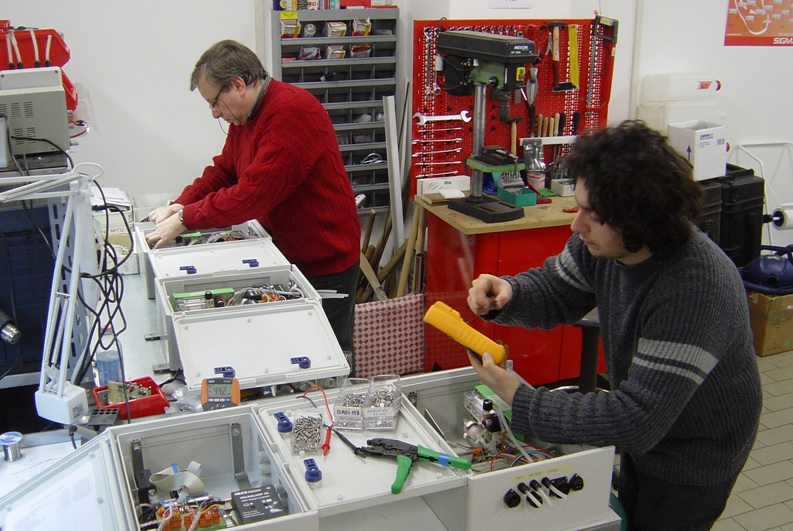
\includegraphics[scale=0.35]{Page1.png}}
				\end{center}
			}
		\end{tabularx}
	\end{frame}
	
	%------------------- Terza slide --------------------
	\begin{frame}{\textbf{La soluzione}}
		\begin{itemize}
			\item L'unione tra i moderni programmi di modellazione 3-D e le nuove tecnologie per la stampa in 3-D permette di risolvere economicamente ed efficacemente il problema.
			\item Inoltre, si tutela l'ambiente aumentando il numero di oggetti che si possono riutilizzare. 
		\end{itemize}
		\vspace*{5mm}
		\begin{center}
			\zoombox{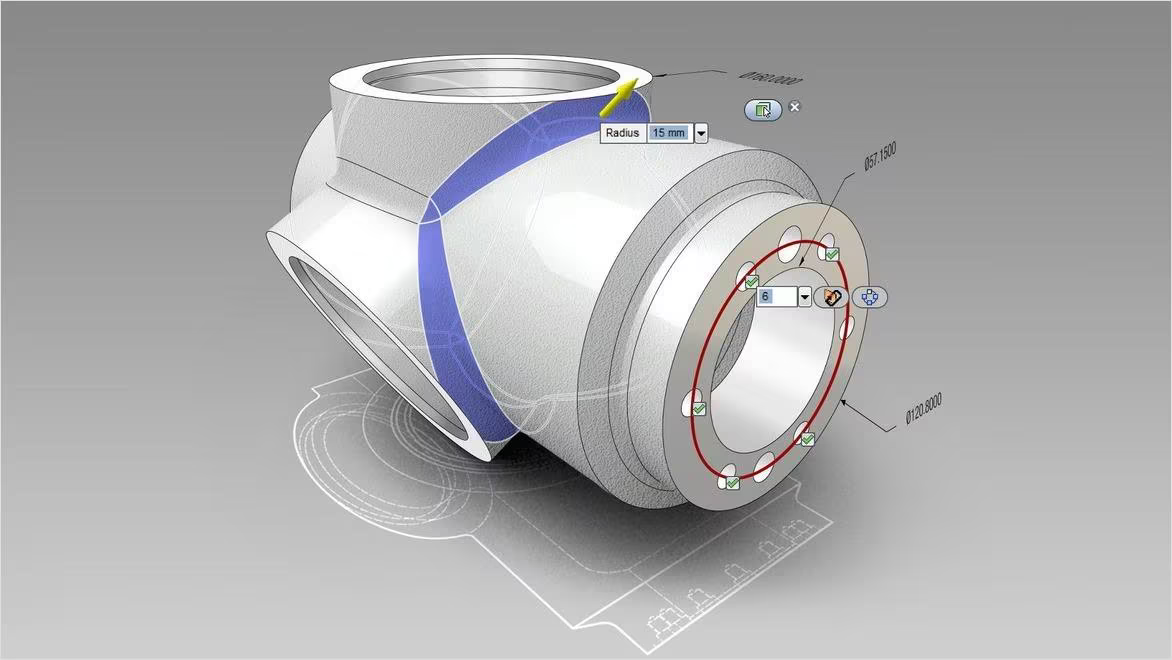
\includegraphics[scale=0.4]{Page2.png}}
		\end{center}
	\end{frame}
	
	%------------------- Quarta slide --------------------
	\begin{frame}{\textbf{Perché ora?}}
		\begin{tabularx}{\linewidth}{XX}
		{
			\begin{center}
					\zoombox{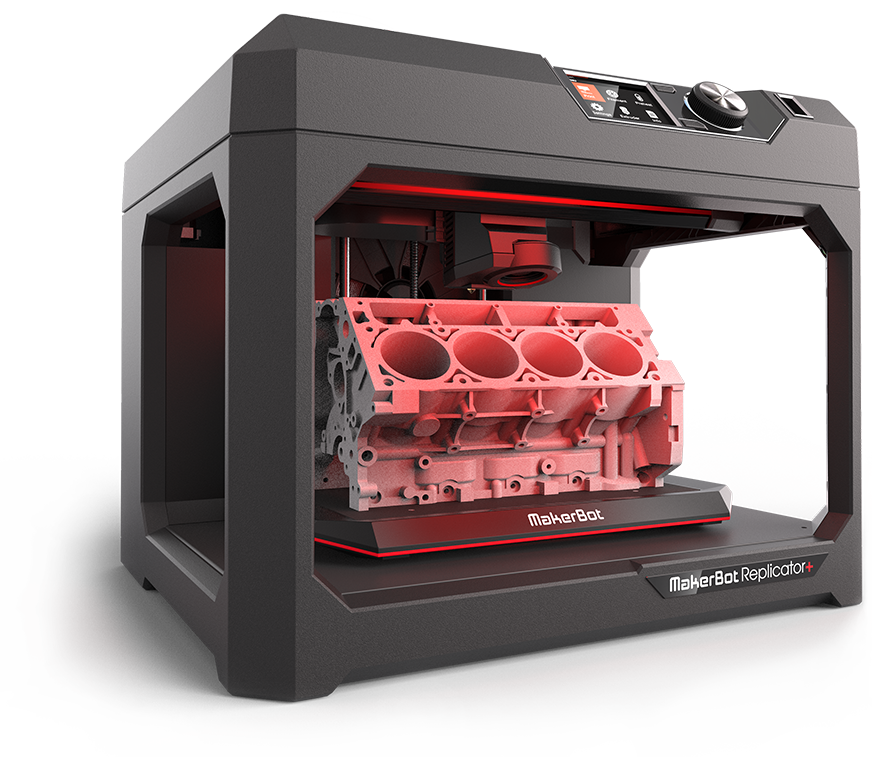
\includegraphics[scale=0.2]{Page3.png}}
			\end{center}
		}&{
			\begin{center}
				\begin{itemize}
					\item Perché è adesso che i programmi di modellazione 3-D hanno raggiunto una espressività tale da permettere facilmente di modellare ogni tipo di pezzo, allo stesso tempo le stampanti in 3-D sono diventante sempre più economiche e avanzate.
				\end{itemize}
			\end{center}
		}		
		\end{tabularx}
	\end{frame}
	
	%------------------- Quinta slide --------------------
	\begin{frame}{\textbf{Potenzialità di mercato}}
		\begin{tabularx}{\linewidth}{XX}
			{
				\begin{center}
					\vspace*{8mm}
					\zoombox{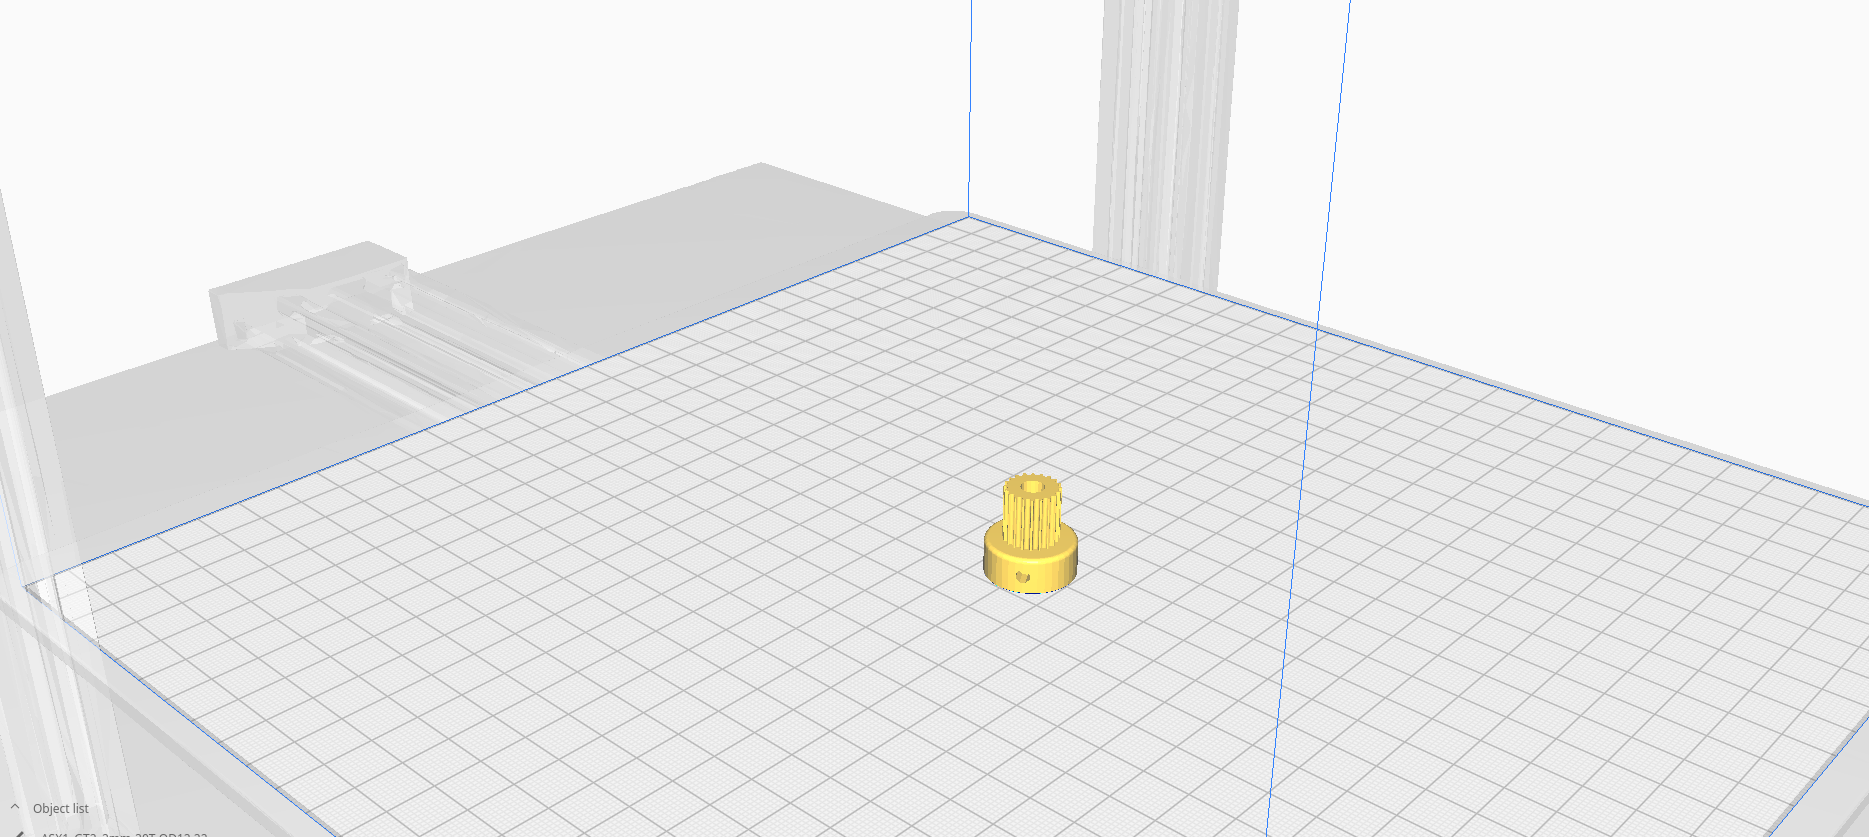
\includegraphics[scale=0.15]{Page4.png}}
				\end{center}
			}&{
				\begin{center}
					\small
					\begin{itemize}
						\item Il costo di modellazione e di stampa di un prototipo si aggira tra i 20€ ed i 30€.
						\item Stampare in una produzione di almeno 50 unità permette di abbassare i costi fino a 8€ il pezzo.
						\item Considerando che gli oggetti sono soggetti ad usura meccanica è facile tenere aperta una piccola produzione costante di parti di ricambio precedentemente modellate.
						\item Il guadagno giornaliero netto di una produzione si aggira attorno ai 15€.
					\end{itemize}
				\end{center}
			}
		\end{tabularx}
	\end{frame}
	
	%------------------- Sesta slide --------------------
	\begin{frame}{\textbf{I concorrenti}}
		\begin{tabularx}{\linewidth}{XX}
			{
				\begin{center}
					\vspace*{15mm}
					\begin{itemize}
						\item Oggi non è più necessario riprodurre le parti di ricambio a mano come una volta facevano gli artigiani.
					\end{itemize}
				\end{center}	
			}&{
				\begin{center}
					\zoombox{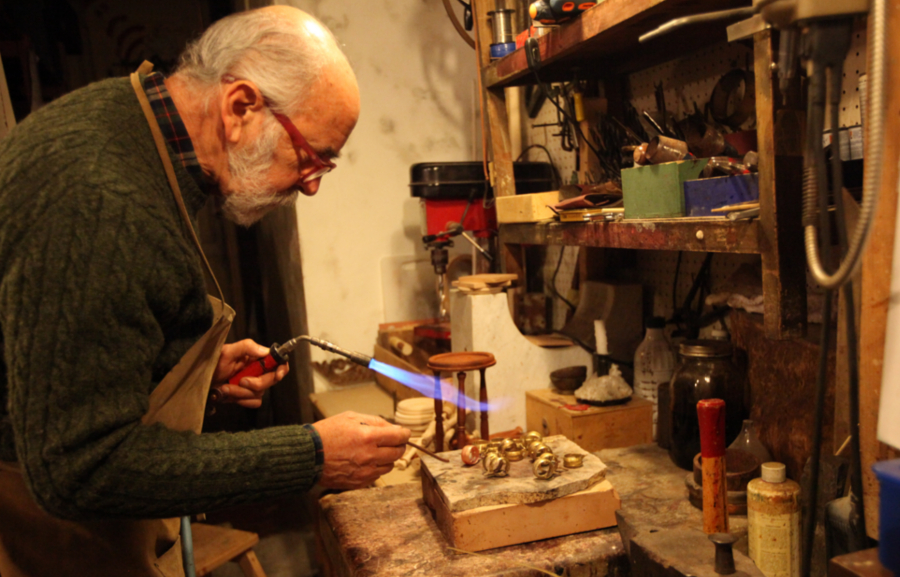
\includegraphics[scale=0.3]{Page5.png}}
				\end{center}
			}
		\end{tabularx}
	\end{frame}

		%------------------- Settima slide --------------------
	\begin{frame}{\textbf{Il business model}}
		\begin{tabularx}{\linewidth}{XX}
			{
			\begin{center}
				\small
				\begin{itemize}
					\item Si prospetta di vendere i prodotti stampati in 3-D prevalentemente ai centri di assistenza, i quali spesso richiedono un numero discreto di elementi che non sono troppo difficili da modellare.
				\end{itemize}
			
				\begin{itemize}
					\item Con una piccola spesa iniziale è già possibile avere una ridotta capacità produttiva.
					\item È facile ingrandire la capacità produttiva, siccome basta semplicemente possedere più macchine che lavorano in parallelo, grazie al fatto che l'infrastruttura di base è fortemente modulare 
				\end{itemize}
			\end{center}
			}&{
				\begin{center}
					\zoombox{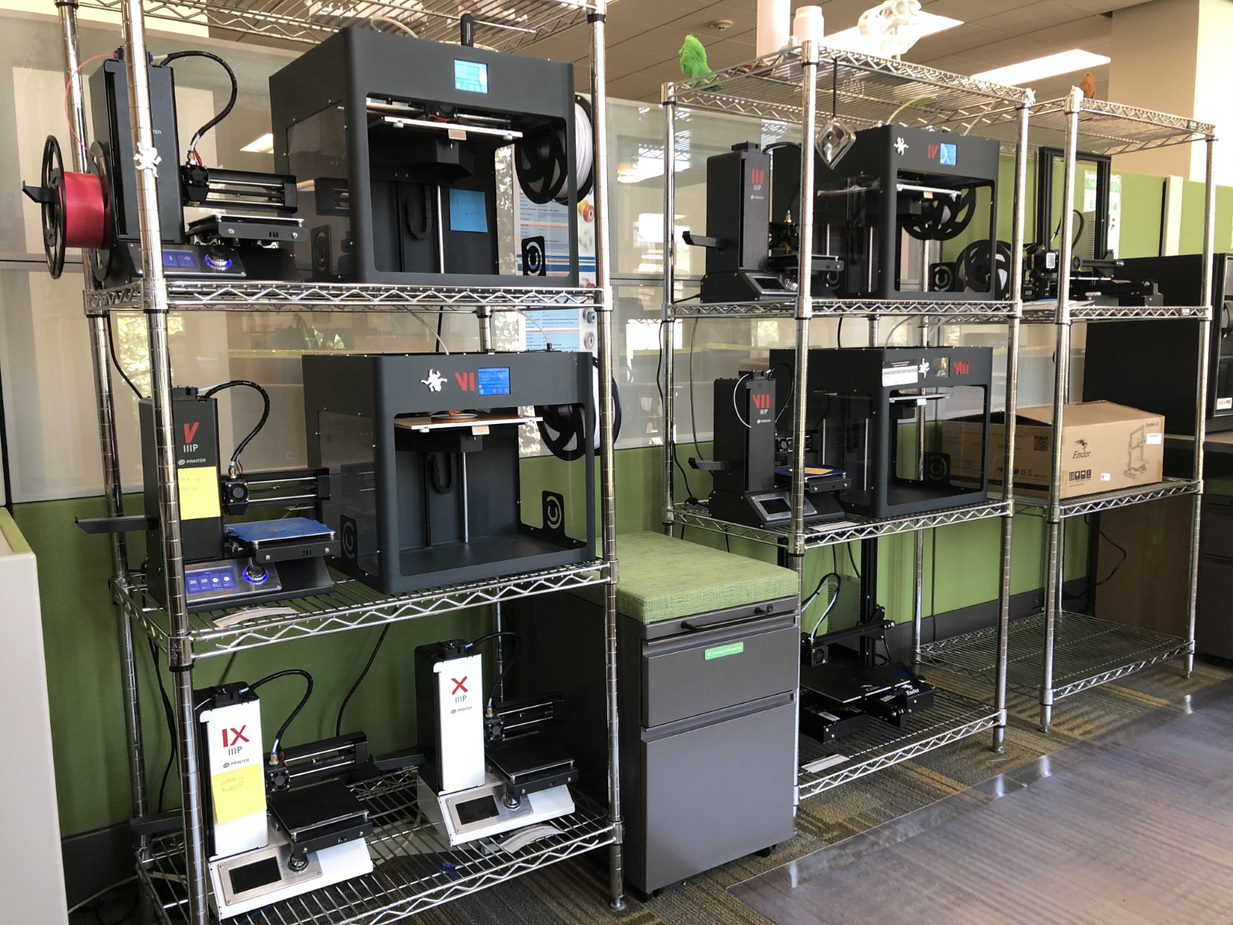
\includegraphics[scale=0.22]{Page6.png}}
				\end{center}
			}
		\end{tabularx}
	\end{frame}
	
	%------------------- Ottava slide --------------------
	\begin{frame}{\textbf{Il team}}
		\begin{itemize}
		
		\item Il team è composto da: \textbf{Francesco Rombaldoni, Rocco Luigi Ciarfaglia e da Marco Belletti}. \newline
		Francesco proveniente dalla facoltà d'informatica, all'interno del team si occupa della messa in opera della stampa in 3-D e di modellare. Rocco, che studia scienze motorie e Marco, studioso di lettere classiche, si occupano di gestire le produzioni, ponendo particolare attenzione alla rifinitura dei modelli. 
		\item Siamo tutti accomunati dal desiderio di utilizzare questa nuova tecnologia per cercare di rendere il nostro ambiente locale un pochino più pulito, riducendo il numero di prodotti che finiscono in discarica a volte anche per piccoli problemi facilmente risolvibili.
		\item Ci siamo conosciuti al Contamination Lab, dove abbiamo stretto velocemente amicizia grazie a questo desiderio in comune. 
			
		%	\item Il team è composto da un gruppo che si occupa di curare la produzione in 3-D, da un altro che si occupa di modellare la parti di ricambio e infine da un reparto marketing. \newline Siamo tutti accumunati dal desiderio di utilizzare questa nuova tecnologia per cercare di rendere il nostro ambiente locale un pochino più pulito, riducendo il numero di prodotti che finiscono in discarica a volte anche per piccoli problemi facilmente risolvibili. \newline
		%	Ci siamo conosciuti al Contamination Lab, dove abbiamo stretto velocemente amicizia grazie a questo desiderio in comune. 
		\end{itemize}
	\end{frame}

	%------------------- Nona slide --------------------
	\begin{frame}{\textbf{Quello che ci serve}}
		\begin{tabularx}{\linewidth}{XX}
			{
				\begin{center}
					\vspace*{7mm}
					\begin{itemize}
						\item Abbiamo bisogno di conoscere tanti centri di assistenza in modo da poter promuovere la nostra idea.
						\item Ma sopratutto, abbiamo bisogno che si prenda consapevolezza che non è necessario buttare ciò che si può riparare!
					\end{itemize}
				\end{center}	
			}&{
				\begin{center}
					\zoombox{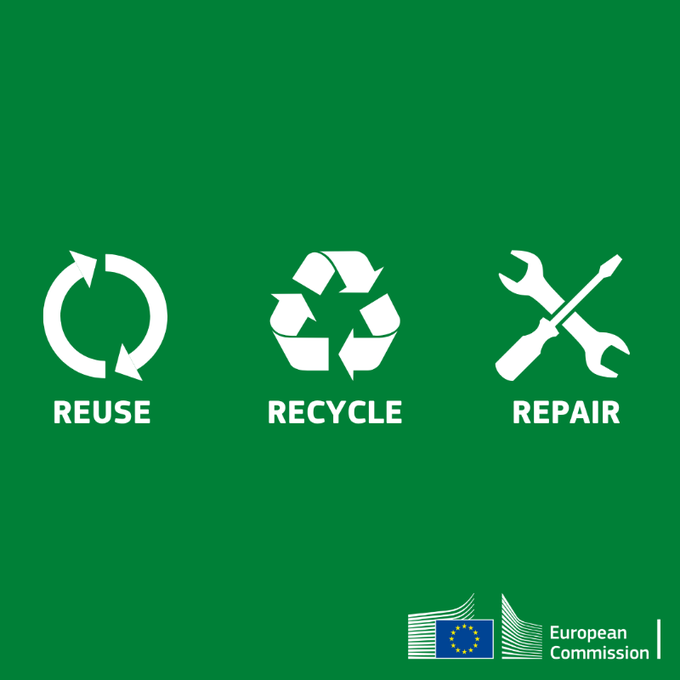
\includegraphics[scale=0.2]{Page7.png}}
				\end{center}
			}
		\end{tabularx}
	\end{frame}
	
	%------------------- Chiusura --------------------

		\begin{frame}[plain]
			\maketitle
			\vspace*{-20mm}
			\begin{center}
				\vspace*{5mm}
				%\newline 
			\begin{tabularx}{\linewidth}{XXX}
				{
					\hspace*{20mm}
					\zoombox{\includegraphics[scale=0.2]{logo_bianco.png}}
				}&{
					\hspace*{8mm}
					\zoombox{
\includegraphics[scale=0.2]{logo-uniurb-2016.jpg}}
				}&{
					\hspace*{10mm}
					\zoombox{
\includegraphics[scale=0.2]{Logo_contamination.png}}
				}
			\end{tabularx}
			
			\vspace{5mm}
			\tiny{\textbf{E-mail: }\href{f.rombaldoni@campus.uniurb.it}{\textcolor{blue}{f.rombaldoni@campus.uniurb.it}} \hspace*{90mm} \textbf{GitHub: }\href{https://github.com/R0mb0}{\textcolor{blue}{R0mb0}} }
			\end{center}
		\end{frame}
	
	% Frame con la licenza
	\begin{frame}
		\vspace*{\fill}
		% Print license shield
		\doclicenseThis
	\end{frame}
	
\end{document}